\section{Math}
\subsection{Hill climbing}
Hill climbing is an useful function to get the maximum value if you don't know what to do!
just make a function and follow the instruction below:
\lstinputlisting{"./codes/math/hill_climbing.cpp"}

\subsection{Linear Seq}
杜教的递推板子,目测大概需要暴力递推阵的大小的两倍。
\lstinputlisting{"./codes/math/linear_seq.cpp"}

\subsection{FFT}
\subsubsection{Bit operation}
$tf(X1,X2) = (tf(X1) - tf(X2), tf(X1) + tf(X2))$

异或:$tf(X1,X2) = (tf(X1) - tf(X2), tf(X1) + tf(X2))$ 

与:$tf(x1,x2)=(tf(x1) + tf(x2), tf(x1))$
\lstinputlisting{"./codes/math/fftbt.cpp"}
\subsubsection{Standard}
\lstinputlisting{"./codes/math/fft.cpp"}
\subsubsection{Usage}
\lstinputlisting{"./codes/math/fft_usage.cpp"}

\subsection{Euler function}
\lstinputlisting{"./codes/math/euler.cpp"}

\subsection{Ex-GCD}
\lstinputlisting{"./codes/math/exGCD.cpp"}
\subsection{M\"obius}
两个公式:
\begin{equation}
F(n) = \sum_{d|n}{} f(d) \Longrightarrow f(n) = \sum_{d|n}{} \mu (d) F(\frac{n}{d}) \tag{1}
\end{equation}
\begin{equation}
F(n) = \sum_{n|d}{} f(d) \Longrightarrow f(n) = \sum_{n | d} \mu (\frac{d}{n})F(d) \tag{2}
\end{equation}
\begin{equation}
\mu(n) = 
\begin{cases}
1 & n = 1\\
(-1)^k & n = p_1 p_2 ... p_k\\
0 & \text{其余情况}
\end{cases}\notag
\end{equation}
\subsubsection{M\"obius用于容斥}
容斥原理:在集合S中至少具有 $P_1 P_2 ... P_m$中一个元素的个数是:
\begin{equation}
|S_1 \cup S_2 \cup S_3 ... \cup S_n| = \sum |S_i| - \sum |S_i \cup S_j| + ... +  \sum (-1) ^ {m + 1} |S_1\cup S_2 ... \cup S_m| \notag
\end{equation}

常用转化式:
\begin{equation}
\sum_{i=1}^{n} \lfloor{\frac{n}{i}}\rfloor = \sum_{i=1}^{n} d(i), d(n)\text{是}n\text{的正因子数目(埃筛)}\notag
\end{equation}

\begin{equation}
[x=1] = \sum_{d|x} \mu (d)\notag
\end{equation}
\lstinputlisting{"./codes/math/mobius.cpp"}
\subsection{Prime}
\subsubsection{Get primes}
\lstinputlisting{"./codes/math/prime.cpp"}
\subsubsection{Get factors}
\lstinputlisting{"./codes/math/factor.cpp"}
\subsubsection{区间筛}
\lstinputlisting{"./codes/math/interval_primes.cpp"}
\subsection{Simpson}
\lstinputlisting{"./codes/math/simpson.cpp"}

\subsection{Chinese remainder theorem}
\lstinputlisting{"./codes/math/chinese.cpp"}

\subsection{Lucas}
\lstinputlisting{"./codes/math/lucas.cpp"}

\subsection{Primitive root}
\lstinputlisting{"./codes/math/getPriRoot.cpp"}
\subsection{Inverse element}
\lstinputlisting{"./codes/math/inverse.cpp"}

\subsection{Calculator}
注意灵活运用。\\
双目运算符在calc()中,左结合单目运算符在P()中,右结合单目运算符在calc\_exp中。(但是还没遇到过。。)\\
\lstinputlisting{"./codes/math/calculator.cpp"}

\subsection{Linear programming}
\lstinputlisting{"./codes/math/lp.cpp"}

\subsection{Factorization prime number p into $x^2+y^2$ }
\lstinputlisting{"./codes/math/fermat.cpp"}

\subsection{Partition ways of an integer}
$O(n\sqrt{n})$
\lstinputlisting{"./codes/math/partition.cpp"}

\subsection{Pell's equation}
\lstinputlisting{"./codes/math/pell.cpp"}

\subsection{Polya}
	设$G$是$p$个对象的一个置换群,用$k$种颜色去染这$p$个对象,若一种染色方案在群$G$的作用下变为另一种方案,则这两个方案当作是同一种方案,这样的不同染色方案数为:\\
	$L=\frac{1}{\left |G  \right |}\times \Sigma(k^{C(f)}), f\in G$\\
	$C(f)$为循环节,$\left |G  \right |$表示群的置换方法数\\
	\\
	对于有$n$个位置的手镯,有$n$种旋转置换和$n$种翻转置换
	\begin{description}
		\item[对于旋转置换:] ~\\
		$C(f_i)=gcd(n,i)$ ,$i$表示一次转过i颗宝石,$i=0$时$c=n$;\\
		\item[对于翻转置换:] ~\\
		\begin{description}
			\item[如果$n$为偶数:] 则有$\frac{n}{2}$个置换$C(f)=\frac{n}{2}$,有$\frac{n}{2}$个置换 $C(f)=\frac{n}{2}+1$\\
			\item[如果$n$为奇数:] $C(f)=\frac{n}{2}+1$\\
		\end{description}
	\end{description}
%\subsection{}
	\subsection{拉格朗日插值法}
	已知$y=a_0+a_1x+a_2x^2+\cdots +a_{n-1}x^{n-1}$曲线上的$n$个点$(x_1,y_1),(x_2,y_2),(x_3,y_3)\cdots (x_n,y_n)$\\
	用拉格朗日插值法可以不求系数可知任意$x$对应的$y$值。\\
	\[ \begin{split}
	y &= y_1\frac{(x-x_2)(x-x_3)\cdots (x-x_n)}{(x_1-x_2)(x_1-x_3)\cdots (x_1-x_n)}\\
	&+ y_2\frac{(x-x_1)(x-x_3)\cdots (x-x_n)}{(x_2-x_1)(x_2-x_3)\cdots (x_2-x_n)}\\
	&+ \cdots \\
	&+ y_n\frac{(x-x_1)(x-x_2)\cdots (x-x_{n-1})}{(x_n-x_1)(x_n-x_2)\cdots (x_n-x_{n-1})}\\
	\end{split}\]
	特别的,如果$x_1\sim x_n$为 连续自然数,那么对于下一个自然数对应的$y$值为:\\
	\[y_{n+1}=(-1)^{n-1}C_n^0y_1+(-1)^{n-2}C_n^1y_2+\cdots +(-1)^0C_n^{n-1}y_n\]
	这个组合系数可以通过高斯消元暴出来,前提是要猜到它满足递推关系。\\
	
	\subsection{正多面体顶点着色}
	正四面体:$N = \frac{(n^{4}+11\times n^{2})}{12}$\\
	正六面体:$N = \frac{(n^{8}+17\times n^{4}+6\times n^{2})}{24}$\\
	正八面体:$N = \frac{(n^{6}+3\times n^{4}+12\times n^{3}+8\times n^{2})}{24}$\\
	正十二面体:$N = \frac{(n^{20}+15\times n^{10}+20\times n^{8}+24\times n^{4})}{60}$\\
	正二十面体:$N = \frac{(n^{12}+15\times n^{6}+44\times n^{4})}{60}$\\
	
	\subsection{求和公式}
	$\sum{k} = \frac{n\times (n+1)}{2}$\\
	$\sum{2k-1} = n^{2}$\\
	$\sum{k^{2}} = \frac{n\times (n+1)\times (2n+1)}{6}$\\
	$\sum{(2k-1)^{2}} = \frac{n\times (4n^{2}-1)}{3}$\\
	$\sum{k^{3}} = (\frac{n\times (n+1)}{2})^{2}$\\
	$\sum{(2k-1)^{3}} = n^{2}\times (2n^{2}-1)$\\
	$\sum{k^{4}} = \frac{n\times (n+1)\times (2n+1)\times (3n^{2}+3n-1)}{30}$\\
	$\sum{k^{5}} = \frac{n^{2}\times (n+1)^{2}\times (2n^{2}+2n-1)}{12}$\\
	$\sum{k\times (k+1)} = \frac{n\times (n+1)\times (n+2)}{3}$\\
	$\sum{k\times (k+1)\times (k+2)} = \frac{n\times (n+1)\times (n+2)\times (n+3)}{4}$\\
	$\sum{k\times (k+1)\times (k+2)\times (k+3)} = \frac{n\times (n+1)\times (n+2)\times (n+3)\times (n+4)}{5}$\\
	$\sum{i\times \binom{n}{i}} = n \times 2^{n - 1}$(子集长度和)\\
	$\sum_{i=1}^{n} \lfloor{\frac{n}{i}}\rfloor = \sum_{i=1}^{n} d(i), d(n)\text{是}n\text{的正因子数目(埃筛)}$\\
	$[x=1] = \sum_{d|x} \mu (d)$
	\subsection{几何公式}
	n-Polygon: $\frac{n}{2} * R ^ 2 * sin( \frac{2 \pi }{n} )$\\
	已知任意三点求边数最少的(同时也是面积最小)正多边形:由于$A=\frac{A'}{2}$ 所以有$A=k \frac{\alpha}{2}$ ,结论: $\alpha = 2gcd(A,B,C)$ 其中A, B, C为三角形内角\\
	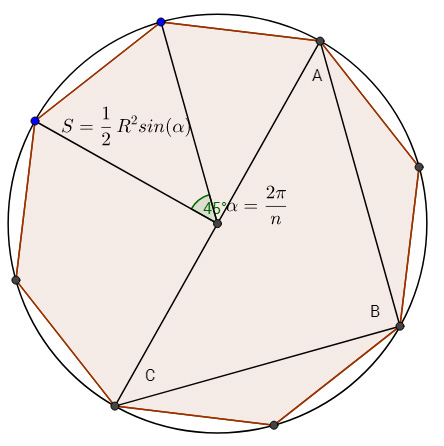
\includegraphics[scale=0.5]{./codes/geometry/npolygon.jpg} 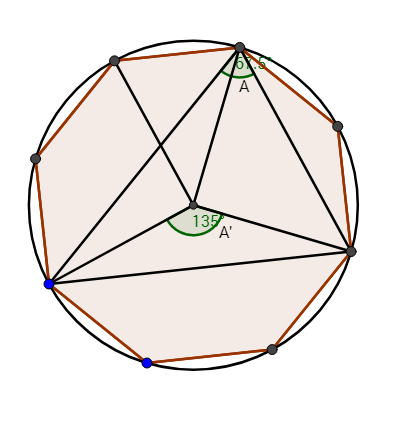
\includegraphics[scale=0.6]{./codes/geometry/npolygon_2.png}\\
	球扇形:\\
	全面积:$T = \pi r(2h+r_0)$,$h$为球冠高,$r_0$为球冠底面半径\\
	体积:$V = \frac{2\pi r^{2}h}{3}$\\
	
	\subsection{小公式}
	Pick 公式:$A = E\times 0.5+I-1$($A$是多边形面积,$E$是边界上的整点,$I$是多边形内部的整点)\\
	\\
	海伦公式:$S = \sqrt{p(p-a)(p-b)(p-c)}$,其中$p = \frac{(a+b+c)}{2}$,$abc$为三角形的三条边长\\
	\\
	求$\binom{n}{k}$中素因子$P$的个数:\\
	\begin {enumerate}
	\item 把$n$转化为$P$进制,并记它每个位上的和为$S1$
	\item 把$n-k$,$k$做同样的处理,得到$S2$,$S3$
	\end{enumerate}
	则$\binom{n}{k}$中素因子$P$的个数:$\frac{S2+S3-S1}{P-1}$\\
	\\
	部分错排公式:\\
	$n+m$个数中$m$个数必须错排 求排列数
	\begin{lstlisting}[language=c++]
dp[i] = n*dp[i-1]+(i-1)*(dp[i-1]+dp[i-2]);
dp[0] = n!;
dp[1] = n*n!;
	\end{lstlisting}
	$dp[m]$为所求解\\
